\subsection{Efficiency of pattern matching}
\label{sec:patternmatchingefficiency}
The design of pattern matching is undoubtedly a strong mechanism for
describing moves, win condition, or any other check that depends on
a particular board layout. Unfortunately, our implementation of the
pattern matching is highly inefficient. Consider the piece placed at
the square D5 in \figref{fig:inefficientpatterns}. The blue piece can
make the moves of a knight from a chess game. This can be specified in
\productname{} with the pattern \texttt{/(n n e|w) | (s s e|w) | (w w
n|s) | (e e n|s) this/}.

\begin{figure}
\centering
\begin{minipage}{.5\textwidth}
  \centering
  \includegraphics[width=.4\linewidth]{pictures/inefficientpatterns}
  \capt{An inefficient implementation.}
  %Pattern matching done on the $8$ green squares will return
  %true, given the moves of a knight and the blue square (D5) as input.
  \label{fig:inefficientpatterns}
\end{minipage}%
\begin{minipage}{.5\textwidth}
  \centering
  \includegraphics[width=.4\linewidth]{pictures/efficientpatterns}
  \capt{An efficient and intuitive implementation.}
  %An efficient and intuitive way to check the moves of a
  %knight piece in a chess game.
  \label{fig:efficientpatterns}
\end{minipage}
\end{figure}

With the current implementation, to find the moves of the piece on D5,
the pattern must be matched on all $64$ squares, given D5 as input.
Those squares for which the pattern matching returns true, are those
squares the piece can move to. In \figref{fig:inefficientpatterns}, only
$8$ of those $64$ checks performed are depicted. For a game of chess
starting with $32$ pieces, the pattern matching is actually done on all
$64$ squares (for all $32$ pieces). If we for simplicity assumed
that each piece had $8$ possible moves, the amount of work related to
pattern checks for the first move in chess can be calculated to be $32
* 64 * 8 = \num{16384}$. Or more generally, $\mathcal{O}(p * n * m *
c)$, where $p = $ the number of pieces, $(n, m) = $ the size of the
gridboard, and $c = $ the complexity of each move. It is easy to see how
inefficient this approach is, so lets now consider a better and more
intuitive approach.

Consider the green piece placed at the square D5 in
\figref{fig:efficientpatterns}. The $8$ arrows show the moves a knight can make.
An easy way to find these squares is simply to start at the knight's square
(D5), move two squares in on of the following directions: north, south, east, or
west, and then one square in an orthogonal direction. This also seems like a
quite efficient approach. This can implemented by modifying the pattern matching
to take a square as input and return a list of squares that satisfy the given
pattern. A pattern for the knight's move could look like \texttt{\%this (n n
e|w) | (s s e|w) | (w w n|s) | (e e n|s)\%}. Notice that the \% $\ldots$
\%-encapsulation is used to distinguish between this modified pattern matching
mechanism from the actual pattern mechanism used in \productname{}, which
encapsulates a pattern between the dots. This modified pattern matching done on
the square D5 would return a list containing the green squares in
\figref{fig:efficientpatterns}, namely the legal moves of a knight on D3.

Compared to the current pattern matching in \productname{}, this approach will
have the complexity $\mathcal{O}(p * c)$. The amount of work related to the
first move of a game of chess would be $32 * 8 = 256$, if we again suppose all
pieces are knights. $256$ is much better than \num{163840} from the previous
example. The complexity here seems to not depend on the actual size of the
gridboard, but this is only true in some cases, e.g.\ when considering the moves
of a knight. If the the moves of a rook are considered, its constant $c$ will
depend on the size of the board for both pattern matching techniques. This is
because a larger board will increase the amount of squares the rook can slide
to. Generally, patterns containing the pattern-value \texttt{*} or \texttt{+}
can have a complexity that depends on the size of the board.

\subsection{Additional functionality with pattern matching}
Many different functionalities could be included in the pattern matching. You
may have noticed the row of black squares in the bottom of the Connect Four game
in \figref{fig:connect4simulated}. These black squares are put there so the
pattern check can allow a piece to be dropped one square north of these squares.
If a pattern keyword \texttt{outofboard} existed that matched a square outside
the board, these squares would not be necessary. A shortcut could also be
considered for specifying patterns of the form \texttt{/(e3) | (w3) | (s3) |
(n3)/}. The \texttt{3} is common, but cannot be used outside parentheses like
\texttt{/(e|w|s|n)3/}, as this means \texttt{/(e|w|s|n) (e|w|s|n) (e|w|s|n)/}.
